\section{Chebyshev Interpolation}

We've seen polynomial interpolation approximate complicated functions
like $\sin(x)$. But the approximation left much to be desired. What's
the solution? Adding more observations? Sometimes this causes more
problems than it solves.

\begin{ex}[Runge phenomena]
  Runge studied polynomial interpolation, and found when he examined a
  function of the form
  \begin{equation}
    f(x) = \frac{1}{1 + 25x^{2}}
  \end{equation}
  on the domain $x\in[-1,1]$. The reason it's $25x^2$ is just to
  exaggerate the effect.

  If we work out by hand the Lagrange polynomial interpolation for
  $f(x)$ on $n=6$ nodes, we find
  \begin{equation}
    P_{6}(x) = \frac{59 - 180 x^{2} + 125 x^{4}}{104}.
  \end{equation}
  We can plot this:
  \begin{center}
    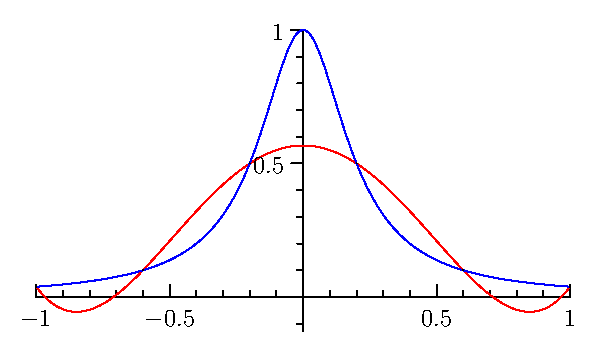
\includegraphics{img/chebyshev.eps}
  \end{center}
  The red curve is the polynomial approximation $P_{6}$, the blue curve
  is the exact $f(x)$.

  % f[x_,n_]:=Sum[g[-1 + 2 k/(n-1)] L[x,n]/ ((D[L[x,n],x] /. x -> (-1 + 2 k/(n-1))) * (x - (-1 + 2 k/(n-1)))), {k,0,n-1}]
  Well, perhaps if we add \emph{more} points to the mesh, accuracy will
  improve? For $n=10$ points, we have
  \begin{equation}
    \begin{split}
    P_{10}(x) =& \frac{74435570719}{86398461344}
    -\frac{356865532425}{43199230672} x^2
    +\frac{331862214375}{10799807668} x^4\\
    &-\frac{1940313234375}{43199230672} x^6
    +\frac{1868347265625}{86398461344} x^8
    \end{split}
  \end{equation}
  Plotting this approximation, we find the situation worsens:
  \begin{center}
    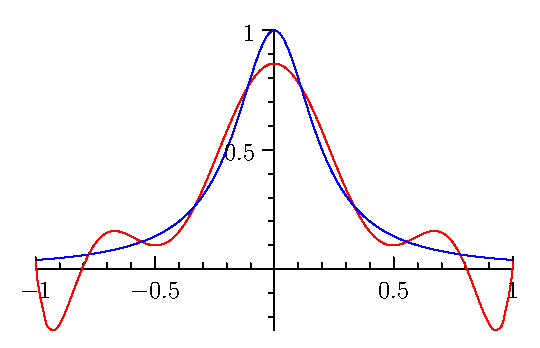
\includegraphics{img/chebyshev2.eps}
  \end{center}
  Why is this happening? Recall Theorem~\ref{thm:interpolation:lagrange:error},
  which told us the error for the Lagrange interpolation for $f(x)$ is
  \begin{equation}
    R_{n}(x) = \frac{f^{(n+1)}(\xi(x))}{(n+1)!}(x-x_{0})(x-x_{1})(\dots)(x-x_{n}).
  \end{equation}
  We selected the points $x_{0}$, $x_{1}$, \dots, $x_{n}$ based off of
  convenience, rather than minimizing this error. Why would we expect
  the error to respect our convenience? Let's try to analyze this error.
\end{ex}

\begin{defn}
  Given some mesh $x_{0}<x_{1}<\dots<x_{n}$, we define the
  \define{Lebesgue Constant}
  \begin{equation}
    \Lambda_{n} = \max_{x_{0}\leq x\leq x_{n}}\prod^{n}_{k=0}|x-x_{k}|.
  \end{equation}
  This can be used to bound the error for polynomial interpolation.
\end{defn}

\begin{ex}
  For $n+1$ equidistant nodes, we see
  \begin{equation}
    \Lambda_{n}\leq n! h^{n+1}
  \end{equation}
  where $h=(b-a)/n$ is the step size. 
\end{ex}

\begin{rmk}
  With Lagrange polynomial interpolation, we see the error is bounded by
  \begin{equation}
    R_{n}\leq f^{(n+1)}(\xi)\frac{h^{n+1}}{n+1}.
  \end{equation}
  Our only hope for small error is that the $(n+1)$-derivative of $f(x)$
  is small.
\end{rmk}

\begin{xca}
  Prove, for $f(x) = (1 + 25 x^{2})^{-1}$ that $|f^{(n+1)}(x)|\leq (n+1)!5^{n+1}$
  (i.e., that $f^{(n+1)}$ is not small).
\end{xca}

\begin{puzzle}
  How can we fix this situation? Or are we doomed with polynomial
  interpolation?\marginpar{I hope one of the lessons you'll learn is: there are no ``no win'' situations.}
\end{puzzle}

We have two factors in the error for polynomial interpolation: the
Lebesgue constant, and the $n+1$ derivative of the interpolant. We can't
control which function we're given to approximate. But perhaps we can
control the Lebesgue constant? After all, we didn't try to minimize the
Lebesgue constant. What mesh could minimize it?

Before answering this question, we need a detour to review some
orthogonal polynomials.

\begin{defn}
  A \define{Chebyshev Polynomial of the First Kind} is
  \begin{equation}
    T_{n}(x) = \cos\bigl(n\arccos(x)\bigr).
  \end{equation}
\end{defn}

\begin{ex}
  From the angle-addition formula
  \begin{equation}
    \cos(x+y)=\cos(x)\cos(y)-\sin(x)\sin(y).
  \end{equation}
  Let $w=\arccos(x)$, then
  \begin{subequations}
  \begin{equation}
    T_{n+1}(x)=\cos\bigl((n+1)w\bigr) = \cos\bigl(nw\bigr)\cos(w)
    - \sin(nw)\sin(w)
  \end{equation}
  and
  \begin{equation}
    T_{n-1}(x)=\cos\bigl((n-1)w\bigr) = \cos\bigl(nw\bigr)\cos(w)
    + \sin(nw)\sin(w).
  \end{equation}
  \end{subequations}
  Thus adding these together give us
  \begin{equation}
    T_{n+1}(x)+T_{n-1}(x)=2xT_{n}(x),
  \end{equation}
  or
  \begin{equation}
    T_{n+1}(x) = 2xT_{n}(x) - T_{n-1}(x).
  \end{equation}
  We see that $T_{0}(x) = 1$, and $T_{1}(x) = x$.
\end{ex}

\begin{prop}
  For each $n$, $T_{n}(x)\in\ZZ[x]$ is a polynomial with integer coefficients.
\end{prop}
\begin{proof}
  We see $T_{0}(x)=1$ and $T_{1}(x)=x$, and if
  $T_{n}(x),T_{n-1}(x)\in\ZZ[x]$, then $2x T_{n}(x) - T_{n-1}(x)$ is a
  linear combination of polynomials with integer coefficients.
  Since $\ZZ[x]$ is closed under addition and subtraction, it follows
  that Chebyshev polynomials are polynomials with integer coefficients.
\end{proof}

\begin{prop}
  The leading coefficient of $T_{n}(x)$ is $2^{n}$.
\end{prop}
\begin{proof}
  This follows from $T_{n+1}(x) = 2xT_{n}(x) + (\mbox{lower order terms})$.
\end{proof}

\begin{prop}
  For any $n$, we see $T_{n}(1)=1$ and $T_{n}(-1) = (-1)^{n}$.
\end{prop}

\begin{prop}\label{prop:interpolation:chebyshev:max-of-chebysev-poly}
  The maximum value of $T_{n}(x)$ is 1, for any $n$.
\end{prop}

\begin{prop}
  All zeroes of $T_{n}(x)$ lie between $-1$ and $+1$.
\end{prop}

\begin{thm}[Chebyshev's Other Theorem]
The choice of real numbers $-1\leq x_{0} < x_{2} < \dots < x_{n}\leq+1$
which minimizes $W_{n}$ is
\begin{equation}
  x_{j} = \cos\left(\frac{(2j-1)\pi}{2(n+1)}\right).
\end{equation}
Further, the minimum value is $2^{-n}$.
\end{thm}
\begin{proof}
  Let $x_{0}$, $x_{1}$, \dots, $x_{n}$ be the roots of
  $T_{n+1}(x)$. Then by the fundamental theorem of algebra,
  \begin{equation}
    \frac{1}{2^{n}}|T_{n+1}(x)| = |(x-x_{0})(\dots)(x-x_{n})|.
  \end{equation}
  By Proposition~\ref{prop:interpolation:chebyshev:max-of-chebysev-poly},
  the maximum value of $T_{n+1}(x)$ is 1, so we have
  \begin{equation}
    |(x-x_{0})(\dots)(x-x_{n})|\leq\frac{1}{2^{n}}.
  \end{equation}
  We now need to show other points cannot lead to a smaller bound.

  Suppose (for contradiction) there is some other mesh which leads to a
  smaller bound.
  Let $P(x)$ be a polynomial whose roots lead to smaller bound. But it
  must satisfy the following properties:
  \begin{enumerate}
  \item The leading term $P(x)\sim x^{n+1}+\bigO(x^{n})$
  \item $|P(x)| < 2^{-n}$ for all $-1\leq x\leq 1$
  \end{enumerate}
  We argue this leads to a contradiction; or, more precisely, that no
  such $P(x)$ can exist.

  Let
  \begin{equation}
    F(x) = P(x) - \frac{T_{n+1}(x)}{2^{n}}.
  \end{equation}
  We see
  \begin{subequations}
    \begin{align}
      F(1) &= P(1) - \frac{1}{2^{n}} < 0\\
      F\left(\cos\left(\frac{\pi}{n}\right)\right)
      &= P\left(\cos\left(\frac{\pi}{n}\right)\right)
      + \frac{1}{2^{n}} > 0\\
      F\left(\cos\left(\frac{2\pi}{n}\right)\right)
      &= P\left(\cos\left(\frac{2\pi}{n}\right)\right)
      - \frac{1}{2^{n}} < 0
    \end{align}
  \end{subequations}
  and so on. There are $n+2$ sign changes for $F$, so there must be $n$
  zeroes for $F$ by the intermediate value theorem. Thus $F$ must be a
  degree $n$ polynomial.

  But $F(x) = P(x) - 2^{-n}T_{n+1}(x)$, so $\deg(F)$ can be no larger
  than $n$.

  Hence we have a contradiction, and we conclude no such $P(x)$ can
  exist. So what? It follows that $2^{-n}T_{n+1}(x)$ is the polynomial
  whose roots minimize the Lebesgue constant.
\end{proof}

\begin{defn}
  Let $n\in\NN$ be a positive integer.
  The \define{Chebyshev nodes} are the $n$ nodes
  \begin{equation}
    x_{k} = \cos\left(\frac{2k - 1}{2n}\pi\right)
  \end{equation}
  for $k=1,\dots,n$.
\end{defn}

\begin{rmk}[Chebyshev interpolation]
  We can use these nodes to do polynomial interpolation. This is
  generically called \emph{Chebyshev interpolation}.
\end{rmk}

\begin{rmk}[History]
  Runge was really studying the exponential function in a clever way. He took
  \begin{equation}
    u := \E^{h}-1
  \end{equation}
  and
  \begin{equation}
    v := x/h
  \end{equation}
  then examined the [truncated] binomial expansion of
  \begin{equation}
    g_{n}(x) = (1 + u)^{v} = 1 + uv + u^{2}\frac{v(v-1)}{1\cdot 2}
    +\dots+u^{n}\frac{v(v-1)(\dots)(v-(n-1))}{1\cdot2\cdot3\cdot(\dots)\cdot n}.
  \end{equation}
  This led him to the function we just examined.
\end{rmk}